\subsection{PCB Meandered Inverted-F Antenna (PIFA)}

PIFA antennas are much more popular in Bluetooth Low Energy stack because of the small size low profile and cost-effective compared to the conventional dipole and ceramic chip antennas.
The proposed structure of the PIFA antenna is routed to gain all these advantages.
Replacing the conventional PCB line in PIFA with the meandering line and meandering shorting strip
improves the efficiency of the PIFA as well as the bandwidth. As a case study, the design and measurement results of the
proposed PIFA are presented \cite{PIFA2017Cheuk} in Figure\ref{fig:PIFA_Antenna_1}.


\begin{figure}[ht]
	\centering
	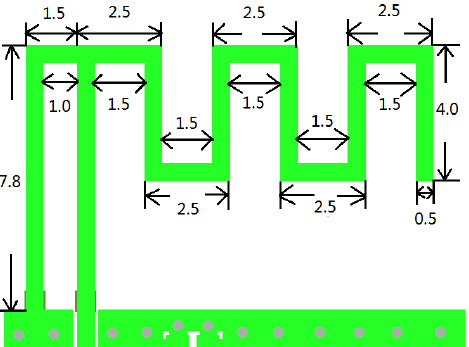
\includegraphics[width=0.65\textwidth]{Chap03/Figures/MIFA_Antenna.PNG}
	\caption{PCB Inverted Meandered F type Antenna }
	\label{fig:PIFA_Antenna_1}
\end{figure}

